\documentclass{article}
\usepackage[utf8]{inputenc}
\usepackage{pdfpages}
% \usepackage[czech]{babel}

\usepackage{geometry}
\geometry{
 a4paper,
%  total={170mm,257mm},
 top=40mm,
 left=30mm,
 right=30mm,
 bottom=25mm
 }

\usepackage{amsmath,amsfonts,amssymb}
\usepackage{enumerate}

\usepackage{subcaption}

% \usepackage{natbib}
%\bibliographystyle{abbrvnat}
% \bibliographystyle{plain}
\bibliographystyle{abbrv}
% \bibliographystyle{amsplain}
% \bibliographystyle{dinat-etal}
% \bibliographystyle{plainnat}
% \setcitestyle{authoryear}

\usepackage[colorlinks=true]{hyperref}

\title{Application of Bayesian Inversion to Characterization of EDZ}
\author{Pavel Exner}
\date{2022}

% \include{math_defs}

\def\abs#1{\lvert#1\rvert}
\def\prtl{\partial}
\def\unit#1{\mathrm{#1}}
\def\bunit#1{[\mathrm{#1}]}
% \def\eps{\varepsilon}
% \def\T{\intercal}
\def\grad{\nabla}
\def\div{\operatorname{div}}
\def\tr{\operatorname{tr}}
\def\vc#1{\mathbf{\boldsymbol{#1}}}     % vector
\def\tn#1{{\mathbb{#1}}}    % tensor
\def\sqr#1{{{\left(#1\right)}^2}}    % tensor

\def\uu{\vc u}
\def\nn{\vc n}
\def\ee{\vc\varepsilon}


\newcommand{\pe}[1]{{\color{red} \textbf{PE: #1}}}
\newcommand{\figpath}{figs/}
\newcommand{\respath}{results/}
\newcommand{\eq}[1]{\begin{equation}{#1}\end{equation}}

\newcommand\figref[1]{Figure~\ref{#1}}
\newcommand\tabref[1]{Table~\ref{#1}}
% reffering subfigure
% \newcommand{\figref}[2][{}]{\hyperref[#2]{\figurename~\ref{#2}#1}} 

\begin{document}

\maketitle

% \section{Introduction}
% Comprehensive models of a~deep geological repository (DGR) for radioactive waste are supposed to describe the transport of radionuclides from the containers through engineering barrier, through geological barrier and into biosphere above the ground for the safety assessment.
% 
% In this contribution we focus ourselves on a~local model of close neighborhood of the boreholes with containers.
% %, i.e. at the interface of engineering and geological barries. Therefore we are deeply interested
% Therefore we are interested in obtaining relevant characteristics of the so-called Excavation Damage Zone (EDZ) which have significant effect on the large-scale transport model parameters, especially hydraulic conductivity and porosity. In our approach we take into account uncertainties in data and we use Bayesian inversion to obtain the model parameters together with their probabilistic properties. This should provide better information to the safety assessment procedures.
% 
% 
% \section{Model}
% 
% Due to lack of data from the current sites in Czechia, we chose to test our approach on the tunnel sealing experiment (TSX) in Canada and compare our results with the deterministic inversion model in~\cite{Rutqvist2009}. The experiment includes measuring water pressure on sides of tunnel during excavation and through one year relaxation period.
% 
% We use our own software \texttt{Flow123d}~\cite{flow123d} to solve the forward 2D hydro-mechanical problem. Above it we use another in-house software \texttt{surDAMH} which implements the Bayesian inversion with Markov chain Monte Carlo sampling according to~\cite{domesova2021efficient}. 
% To decrease the computational costs, the \emph{Delayed acceptance Metropolis-Hastings} algorithm with surrogate model is used.


\subsection{Forward hydro-mechanical model}

Let us consider the geometry as a~2D manifold in arbitrary 3D space.

\subsubsection{Governing equations}

\paragraph{Mechanical model.}
Deformation of the porous media is modelled by the stationary linear elasticity equation
\eq{ \label{eq:lin_el} -\div(\tn \sigma(\uu)) = \vc f + \vc f_H. }
Here $\uu$ $\bunit{m}$ is the displacement vector field with 3 components, the stress tensor is given by the Hooke law
\eq{ \tn\sigma(\uu) = \tn C\ee(\uu) = 2\mu\ee(\uu) + \lambda(\tn I:\ee(\uu))\tn I, }
and the Lam\'e parameters are determined in terms of the Young modulus $E$ $\bunit{Pa}$ and Poisson's ratio $\nu$ $\bunit{-}$:
\eq{ \mu = \frac{E}{2(1+\nu)},\quad \lambda = \frac{E\nu}{(1+\nu)(1-2\nu)}. }
The strain tensor in $\Omega$ is defined as follows:
\eq{ \ee(\uu) = \frac12(\nabla\uu+\nabla\uu^\top). }
The symbol $\vc f$ stands for the body load $\bunit{{N\cdot m}^{-3}}$ and $\vc f_H$ plays a~role in the hydro-mechanical coupling,
see \eqref{eq:mech_fluid_source}.


\paragraph{Flow model.}
We consider the Darcy's law for flow in porous media in the form
\eq{ \label{eq:darcy_flux} \vc q = - \delta\tn K \grad h, } %\qquad\text{in }\Omega_d,\ \text{for $d=1,2,3$}. }
where $\tn K$ $\bunit{m\cdot s^{-1}}$ is the hydraulic conductivity tensor, $h$ $\bunit{m}$ is the hydraulic pressure head and $\delta$~$\bunit{m}$ is the thickness of the 2D domain.

The continuity equation for saturated porous medium then takes the form
\eq{ \label{eq:continuity}
    \prtl_t (\delta S_s\, h) + \div \vc q = F + F_M. } %\qquad \text{in }\Omega_d,\ \text{for $d=1,2,3$},}
where  $S_s$ $\bunit{m^{-1}}$ is the specific storage and $F$ $\bunit{m\cdot s^{-1}}$ is 
the source term. The extra source term $F_M$ $\bunit{m\cdot s^{-1}}$ due to mechanics is defined later by \eqref{eq:fluid_source_div_u}. In our setting the principal unknowns of the system \eqref{eq:darcy_flux} and \eqref{eq:continuity} are both $h$ and $\vc q$ (discretization using Lumped Mixed Hybrid Method).

\paragraph{Hydro-mechanical coupling.}
The mechanics equation \eqref{eq:lin_el} is coupled to flow by the term
\eq{ \label{eq:mech_fluid_source} \vc f_H = -\nabla(\delta\alpha p), \quad p = \varrho_l g h, }
where $p$ $\bunit{Pa}$ is the pressure, $\alpha$ $\bunit{-}$ is the Biot coefficient, $\varrho_l$ $\bunit{kg\cdot m^{-3}}$ is the fluid density and $g$ $\bunit{m\cdot s^{-2}}$ is the gravitational acceleration.
Conversely, the deformation affects the flow via the additional term
\eq{ \label{eq:fluid_source_div_u} F_M = -\partial_t(\delta\alpha\div\uu) }
on the right hand side of \eqref{eq:continuity}.
% The expression $\widetilde\div\uu$ is defined as follows:
% \[ \widetilde\div\uu_d = \div\uu_d + \begin{cases}\frac{\delta_{d+1}}{\delta_d}\sum_{i=1}^n\uu^i_{d+1}\cdot\nn^i_{d+1} & \mbox{ if }d\in\{1,2\},\\0 & \mbox{ else. }\end{cases} \]
The numerical solution of coupled hydro-mechanical problems is solved by an iterative splitting, where in order to achieve convergence the flow equation is modified as follows:
\eq{ \partial_t(\delta(S+S_{extra})\,h) + \div\vc q = F + F_M + \partial_t(\delta S_{extra} h_{old}). }
Here $h_{old}$ is the previous value of piezometric head in the iteration process and $S_{extra}$ is an extra storativity coefficient whose value affects the rate of convergence.

\subsubsection{Forward Model 1 -- simplest setting}
\label{sec:model_01}
We list the common values of the elementary parameters, i.e. fluid density, gravitational acceleration and 2D domain cross-section: 
\[\varrho_l=1000\,\unit{kg\cdot m^{-3}},\; g=9.81\,\unit{m\cdot s^{-2}} \mbox{ and } \delta=1\,\unit{m}.\]
The geometry is shown in \figref{fig:model_01_geometry} and boundary conditions are depicted.
The input parameters of the fixed forward model are gathered in \tabref{tab:model_01_parameters}.

\begin{figure}[!htb]
    \centering
    \includegraphics[width=0.9\textwidth]{\figpath geometry_bc2.pdf}
    \caption{Model geometry of the tunnel 2D cross-section with boundary condition depicted.}
    \label{fig:model_01_geometry}
\end{figure}

The excavation during first 17 days is simulated through the inner boundary condition on the tunnel surface.
Pressure head is linearly decreased from the initial pressure head to zero (atmospheric pressure head after excavation).
The mechanical stress change during excavation is provided by linear increase of stress to the value of the initial stress
(there is no supporting material in the tunnel area after excavation).

\begin{table}[!htb]
    \centering
    \begin{tabular}{|lllc|}
        \hline
        parameter & symbol & value & unit \\
        \hline
        hydraulic conductivity & $K$ & $5.886\cdot10^{-15}$ & $\unit{m\cdot s^{-1}}$ \\
        storativity & $S$ & $7.291\cdot10^{-8}$ & $\unit{m^{-1}}$ \\
%                 \hfill $S=\rho g(\beta_s + \vartheta \beta_w)$ \\
%           \begin{itemize}
%             \item kompresibilita horniny $\beta_s = 0$ $\mathrm{[Pa^{-1}]}$
%             \item kompresibilita vody $\beta_w = 4\cdot 10^{-10}$ $\mathrm{[Pa^{-1}]}$
%             \item porozita $\vartheta = 0.007$ $\mathrm{[-]}$
%           \end{itemize}
    %
        initial pressure head & $h_0$ & $300$ & $\unit{m}$ \\
        Biot-Willis coeffiecient & $\alpha$ & $0.2$ & $\unit{-}$ \\
        Young modulus & $E$ & $6\cdot10^{10}$ & $\unit{Pa}$ \\
        Poisson ratio & $\nu$ & $0.2$ & $\unit{-}$ \\
    \hline
    \end{tabular}
    \caption{Forward model input parameters.}
    \label{tab:model_01_parameters}
\end{table}

% http://hydrogeologistswithoutborders.org/wordpress/1979-english/chapter-2/#2.8

Hydraulic conductivity depends on permeability $k$, dynamic viscozity $\mu = 0.001\,\bunit{Pa\cdot s}$, fluid density and gravity
\eq{K = \frac{k\rho_l g}{\mu}
% = \left[\frac{\unit{m^2}\cdot\unit{kg\cdot m^{-3}}\cdot\unit{m\cdot s^{-2}}}{\unit{Pa\cdot s}}\right].
\qquad \approx 5.886\cdot10^{-15}\,\unit{m\cdot s^{-1} \mbox{ for } k = 6\cdot10^{-22}\,\unit{m^2}}.
}
%
Storativity $S\,\bunit{-}$ depends on the following quantities
\eq{S = \delta S_s = \delta \rho g \left(\beta_s + \eta \beta_w\right)}
% = 3.28\cdot10^{-7}$,
where $\eta$ $\bunit{-}$ is porosity, $\beta_w$ $\bunit{Pa^{-1}}$ compressibility of fluid phase and
$\beta_s$ $\bunit{Pa^{-1}}$ \pe{compressibility of solid grains} of porous media which can be derived
% \eq{\mbox{WRONG (low storativity):} \qquad \beta_s = 0}
% \eq{\mbox{WRONG (high storativity):}\qquad \beta_s = \frac{1}{K_s} = \frac{3(1-2\mu)}{E}}
\eq{ \beta_s = \frac{(\alpha-\eta)(1-\alpha)}{K} }
%
By substituting parameters from \tabref{tab:model_01_parameters}, we get
\eq{ S = 9.81\cdot10^3\left((0.2-0.007)(1-0.2)\cdot 3\cdot10^{-11}
+ 7\cdot10^{-3} \cdot 4\cdot10^{-10}\right) \approx 7.291\cdot10^{-8}}

\begin{figure}[!htb]
    \centering
    \includegraphics[width=0.75\textwidth]{\respath fixed_model/fixed_01/observe_comparison.pdf}
    \caption{Results of Model 1 -- observed pressure.}
    \label{fig:model_01_observe_pressure}
\end{figure}

% \pe{We are not sure about the reduction from 3D to 2D model.
% \begin{itemize}
%     \item We consider all our quantities and equations in 3D space (displacement -- vector of 3 components, stress -- tensor $3\times3$).
%     \item Due to boundary conditions, we obtain zero deformation in $z$-axis.
%     \item Due to 3D tensor, we obtain nonzero $\sigma_{33}\neq0$, the shear stresses $\sigma_{13}=\sigma_{23}=0$ due to b.c.
%         We set $\sigma_{33}=0$ as initial value.
%     \item We did not prescribe any forces in $z$-axis. The results are qualitatively comparable with ZM, although the 
%         the peak of HGT1-5 cannot be reached.
%     \item We have Young modulus and $x$ stress absolutely unrealistic in Bayes aposterior (see best fits below), needs to be recomputed.
% \end{itemize}
% }



\subsubsection{Model 2 -- nonlinear hydraulic conductivity}
The second model is derived directly from Model 1 (Section \ref{sec:model_01}).
We consider the same geometry and parameters with the only difference in hydraulic conductivity.

\paragraph{Nonlinear hydraulic conductivity.}
Empirical nonlinear dependence of hydraulic conductivity on stress:
\eq{ K = \frac{\rho g}{\mu} \left[\mathring{k}_r + \Delta \mathring{k}_m\exp(\mathring\beta\sigma_m)\right]\exp(\mathring\gamma\Delta\sigma_{VM}) }
where
\begin{itemize}
    \item $\mathring k_r=2\cdot10^{-21}\unit{m^2}$ is \emph{residual (irreducible) permeability at high compressive mean stress}
    and the fitting constants are: $\Delta \mathring{k}_m=8\cdot10^{-17}\unit{m^2}$,  $\mathring\beta=4\cdot10^{-7}\unit{Pa^{-1}}$, $\mathring\gamma=3\cdot10^{-7}\unit{Pa^{-1}}$
    \item the mean of the principal stresses, i.e.
        \eq{\label{eq:mean_stress} \sigma_m:=\frac13\tr\tn\sigma(\uu)}
    \item von Mises stress
        \eq{\label{eq:von_mises} \sigma_{VM}:=\sqrt{\frac32\tn\sigma_d:\tn\sigma_d} 
            = \frac{1}{\sqrt{2}}\sqrt{\sqr{\sigma_1-\sigma_2}+\sqr{\sigma_2-\sigma_3}+\sqr{\sigma_1-\sigma_3}},}
        where $\tn\sigma_d:=\tn\sigma(\uu)-\frac13(\tr\tn\sigma(\uu))\tn I$ is the deviatoric stress;
    \item $\Delta\sigma_{VM}$ is understood as the \emph{non-negative} difference between the computed $\sigma_{VM}$ and
        \emph{a critical deviatoric stress for onset of shear-induced permeability}, $\sigma_{c}$, by~\cite{rutqvist_fractured_2015}.
        Let us denote
        \eq{\Delta\sigma_{VM} = \max\left(0, \sigma_{VM} - \sigma_{c}\right),}
        with $\sigma_{c}=55\,\unit{MPa}$.
\end{itemize}

\begin{figure}[htb!]
    \centering
    \begin{subfigure}[t]{0.495\textwidth}
      \includegraphics[width=\textwidth]{\respath fixed_model/fixed_02/observe_comparison.pdf}
      \caption{Coarse mesh.}
      \label{fig:mass_mobile_flow123d}
    \end{subfigure}
    \begin{subfigure}[t]{0.495\textwidth}
      \includegraphics[width=\textwidth]{\respath fixed_model/fixed_03/observe_comparison.pdf}
      \caption{Fine mesh.}
      \label{fig:mass_sorbed_flow123d}
    \end{subfigure}
    \caption{Results of Model 2 -- observed pressure, nonlinear conductivity.}
    \label{fig:balance_flow123d}
\end{figure}

% The geometry is shown in \figref{fig:model_01_geometry} and boundary conditions are depicted.
% The input parameters of the fixed forward model are gathered in \tabref{tab:model_01_parameters}.

% \begin{figure}[!htb]
%     \centering
%     \includegraphics[width=0.9\textwidth]{\figpath geometry_bc2.pdf}
%     \caption{Model geometry of the tunnel 2D cross-section with boundary condition depicted.}
%     \label{fig:model_01_geometry}
% \end{figure}
% 
% 
% \begin{table}[!htb]
%     \centering
%     \begin{tabular}{|lllc|}
%         \hline
%         parametr & symbol & hodnota & jednotka \\
%         \hline
%         vodivost & $K$ & $6\cdot10^{-15}$ & $\mathrm{m\cdot s^{-1}}$ \\
%         storativita & $S$ & $2.8\cdot10^{-8}$ & $\mathrm{m^{-1}}$ \\
% %                 \hfill $S=\rho g(\beta_s + \vartheta \beta_w)$ \\
% %           \begin{itemize}
% %             \item kompresibilita horniny $\beta_s = 0$ $\mathrm{[Pa^{-1}]}$
% %             \item kompresibilita vody $\beta_w = 4\cdot 10^{-10}$ $\mathrm{[Pa^{-1}]}$
% %             \item porozita $\vartheta = 0.007$ $\mathrm{[-]}$
% %           \end{itemize}
%     %
%         počáteční tlaková výška & $h_0$ & $300$ & $\mathrm{m}$ \\
%         Biotův koef. & $\alpha$ & $0.2$ & $\mathrm{-}$ \\
%         Youngův modul & $E$ & $6\cdot10^{10}$ & $\mathrm{Pa}$ \\
%         Poissonovo č. & $\nu$ & $0.2$ & $\mathrm{-}$ \\
%     \hline
%     \end{tabular}
%     \caption{}
%     \label{tab:model_01_parameters}
% \end{table}

% \pe{We are not sure, how to perform the reduction from 3D to 2D model.
% \begin{itemize}
%     \item $\sigma$ is the effective stress throughout this text (should be consistent with relations \eqref{eq:mean_stress} and \eqref{eq:von_mises}).
%     \item Do we understand correcly the critical deviatoric stress $\sigma_{c}$ from Rutquist?
%     \item Should we include the third component of the stress $\sigma_{33}$ in the initial value?
%     \item Should we include $\sigma_3$ into the computation of the hydraulic conductivity?
% \end{itemize}
% }



\section{Results}
In Figure \ref{fig:histograms} we demonstrate an example visualization of the results by means of marginal histograms. We see the comparison of prior (orange) and posterior (blue) probabilistic distribution on the diagonal. From the 2D histograms of the parameter pairs we can see significant correlation between hydraulic conductivity and storativity for example and also for pair Young modulus and initial stress i $x$-axis. The best-fit samples are denoted by red dot.


\begin{figure}[!htb]
    \centering
    \includegraphics[width=0.75\textwidth]{\respath 4par}
    \caption{1D and 2D marginal histograms.}
    \label{fig:histograms}
\end{figure}

\newpage
% \vspace{-15pt}
% \section*{References}
% \renewcommand{\section}[2]{}%
% \section{References}
\bibliography{biblio.bib}



\end{document}
